% SPDX-License-Identifier: Apache-2.0
\documentclass[11pt,letterpaper]{article}
\usepackage[margin=0.82in,headheight=16pt]{geometry}
\usepackage{fontspec}
\setmainfont{P052-Roman}[BoldFont=P052-Bold,ItalicFont=P052-Italic,BoldItalicFont=P052-BoldItalic]
\setsansfont{DejaVu Sans}
\setmonofont[Scale=0.84]{DejaVu Sans Mono}
\usepackage{amsmath,amssymb,booktabs,longtable,array,tabularx,microtype,enumitem}
\usepackage[dvipsnames]{xcolor}
\usepackage{tikz,pgfplots}
\pgfplotsset{compat=1.18}
\usetikzlibrary{positioning,calc}
\usepackage{fancyhdr,titlesec,float}
\usepackage[unicode,colorlinks=true,linkcolor=RoyalPurple,urlcolor=RoyalPurple,citecolor=RoyalPurple]{hyperref}
\usepackage{bookmark}
\definecolor{cosmic}{HTML}{211035}
\definecolor{violet}{HTML}{6A34A3}
\definecolor{lavender}{HTML}{F2ECF8}
\definecolor{gold}{HTML}{EAC980}
\definecolor{ink}{HTML}{271D39}
\definecolor{muted}{HTML}{695C79}
\definecolor{good}{HTML}{276955}
\definecolor{rose}{HTML}{9F3159}
\color{ink}
\hypersetup{pdftitle={The Next Upgrade: An AGI ALPHA Business Case for Consumer-Specific Dependency Decisions},pdfauthor={AGI ALPHA Research},pdfsubject={Useful work, reproducible dependency assessment, and complete-cost investment qualification},pdfkeywords={AGI ALPHA, TRANSFORMATIONAL INTELLIGENCE, SUCCESSOR, dependency upgrade, economics, reproducibility},pdfstartview={}}
\titleformat{\section}{\Large\sffamily\bfseries\color{violet}}{\thesection}{0.7em}{}
\titleformat{\subsection}{\large\sffamily\bfseries\color{ink}}{\thesubsection}{0.7em}{}
\titlespacing*{\section}{0pt}{20pt}{9pt}
\titlespacing*{\subsection}{0pt}{15pt}{7pt}
\setlength{\emergencystretch}{3em}
\setlength{\parindent}{0pt}\setlength{\parskip}{6pt}
\setlist[itemize]{leftmargin=1.3em,itemsep=2pt,topsep=3pt}
\setlist[enumerate]{leftmargin=1.6em,itemsep=3pt,topsep=4pt}
\renewcommand{\arraystretch}{1.2}
\pagestyle{fancy}\fancyhf{}
\fancyhead[L]{\sffamily\small\color{muted}AGI ALPHA $\infty$ \quad THE NEXT UPGRADE}
\fancyhead[R]{\sffamily\small\color{muted}RESEARCH EDITION · 26 OCT 2026}
\fancyfoot[R]{\sffamily\small\thepage}
\renewcommand{\headrulewidth}{0.3pt}
\newcommand{\pathcode}[1]{{\small\ttfamily\detokenize{#1}}}
\newcommand{\unknown}{\textit{Unknown}}
\newcolumntype{Y}{>{\raggedright\arraybackslash}X}
\newcommand{\ConvAccepted}{12}
\newcommand{\CustomAccepted}{9}
\newcommand{\IncMedian}{0.164}
\newcommand{\CustomMedian}{12.018}
\newcommand{\ConvMedian}{12.421}
\newcommand{\CampaignWall}{886.053}
\newcommand{\CampaignCPU}{887.619}
\begin{document}
\begin{titlepage}
\thispagestyle{empty}
\begin{tikzpicture}[remember picture,overlay]
\fill[cosmic] (current page.south west) rectangle (current page.north east);
\draw[white,opacity=.08,line width=1pt] ($(current page.north east)+(-0.8in,-2.0in)$) circle (2.3in);
\draw[white,opacity=.06,line width=1pt] ($(current page.north east)+(-0.8in,-2.0in)$) circle (3.0in);
\foreach \x/\y/\r in {1/1/1,2.3/2/0.8,5.4/1.3/0.6,6.7/3.8/1,1.4/5.3/0.6,4.8/6/0.8,6.4/7.5/0.7}{\fill[gold,opacity=.5] ($(current page.north west)+(\x in,-\y in)$) circle (\r pt);}
\end{tikzpicture}
\color{white}
{\sffamily\bfseries\large AGI ALPHA $\infty$\par}
\vspace{0.2in}
{\sffamily\small\color{gold} THE VALUE THAT COMPOUNDS\par}
\vspace{0.65in}
{\fontsize{48}{52}\selectfont The Next\\Upgrade\par}
\vspace{0.24in}
{\Large A business case for consumer-specific\\dependency decisions\par}
\vspace{0.5in}
{\large\color{gold} Start with a useful result.\par}
{\large An exact failing call. A known remedy reproduced.\\A reusable offering tested on new source revisions.\par}
\vspace{0.55in}
\begin{tabularx}{\textwidth}{@{}YYY@{}}
{\sffamily\bfseries\LARGE 1} & {\sffamily\bfseries\LARGE \ConvAccepted/12} & {\sffamily\bfseries\LARGE 0}\\
Historical incident reproduced & Conventional scoped packets accepted & Actual customer collections\\
\end{tabularx}
\par\vspace{0.35in}
{\normalsize The engineering result is inspectable. Complete delivery cost, a matched human duration, a validated price and investment repayment remain unestablished.\par}
\vfill
{\small\sffamily AGI ALPHA Research · Independent complementary research lane\\
Prepared through AI-assisted engineering and separate same-session review\\
26 October 2026 · Source and protocol frozen before confirmation acquisition\par}
\vspace{0.2in}
{\footnotesize\color{gold} TRANSFORMATIONAL INTELLIGENCE $\infty$ \quad SUCCESSOR $\Omega$ / Harness\par}
\end{titlepage}

\section*{Executive finding}
\addcontentsline{toc}{section}{Executive finding}
A Python maintainer needs to know what a proposed dependency update changes for the project, which calls deserve attention and what to test next. We built a local AGI ALPHA offering that delivers a source-pinned decision packet, verified argument-binding witnesses, a census of captured consumer calls, explicit unresolved cases and downloadable evidence. It uses the existing TRANSFORMATIONAL INTELLIGENCE source inventory and the SUCCESSOR Workbench extension, rather than introducing a competing executor or financial system.

The strongest completed example concerns a real, previously reported HTTPX/Starlette incompatibility. The original dependency pair returns the expected HTTP 200 response. Changing HTTPX alone reproduces the actual \pathcode{TypeError}; the known upstream Starlette remedy restores the identical minimal response. The packet connects that outcome to \pathcode{starlette/testclient.py:429}, the \pathcode{app} argument, exact environment locks and an offline replay. This is exposed historical development, not autonomous repair invention or fresh customer demand.

After bounded discovery and an exact public freeze, we evaluated twelve distinct historical release transitions across Requests, FastAPI and urllib3. A conventional method built with Griffe and independently constructed binding witnesses produced \ConvAccepted/12 independently accepted scoped packets. The custom constraint method produced \CustomAccepted/12. Its rejected reports disagree with the evaluator's conservative treatment of assignments through class objects; separate diagnosis found no lost binding in the disputed signatures. The primary rejection remains in place. No affected consumer call was established on the confirmation transitions. Three lost call shapes occurred in FastAPI helper declarations; they do not establish three defects, a public-API promise violation or a customer outage.

\textbf{The contribution is a working, bounded decision-support offering and a disciplined selection of the stronger available implementation. Commercial superiority is not established.} The complete monetary cost, matched human service duration, customer price, remaining customer effort and paid utilization are unknown. Actual collections are zero. The canonical economic ledger therefore does not admit a self-financing investment. This is a distinct engineering advance toward an automated service, with a concrete commercial test still required.

\section{The buyer's job and the offer}
\subsection{A concrete deliverable}
The buyer hypothesis is a maintainer or engineering lead responsible for a Python service and a proposed dependency change. The recurring need is compatibility triage when a dependency revision, consumer revision or substantive requirement changes. A source-identical repeated request is a no-op. Each accepted packet must identify its exact input scope, account for every changed Python module, distinguish upstream declaration changes from actual captured uses, validate any lost-binding witness and state the next review or integration-test action. It must never present unresolved source or runtime behavior as a compatibility clearance.

\begin{table}[H]\small
\begin{tabularx}{\textwidth}{@{}p{1.35in}Y@{}}\toprule
Buyer input & Finished output and decision enabled\\\midrule
Old/new dependency commits; permitted consumer snapshot & Reconciled source identities and changed-module inventory. The maintainer can verify which revisions were assessed.\\
Captured consumer scope & Exact supported call sites, source lines and argument shapes; unresolved imports, expansions and dispatch remain visible.\\
Proposed transition & Independently checked binding counterexamples, broader Griffe alerts, before/after evidence and a bounded next action.\\
Acceptance requirement & Machine-readable packet plus English/French presentation, reproducible commands and complete-cost unknowns.\\\bottomrule
\end{tabularx}
\caption{The offered service is a bounded compatibility decision aid. It does not perform a whole application migration or authorize a deployment.}
\end{table}

The human work it could replace is part of source comparison, caller search, construction of a minimal compatibility check and preparation of review evidence. A competent maintainer may already use Git, Griffe, dependency-update tools, cached environments and project tests. Those tools and project knowledge are legitimate alternatives. Professional responsibility, behavioral testing, customer context and final release acceptance are not assumed to disappear.

\subsection{Need, recurrence and demand are different facts}
The project declares and uses the dependency ecosystem examined here, and a public Starlette discussion documents a real blocked TestClient workflow after an HTTPX change \cite{starlette-discussion,httpx-release}. Published source histories provide observable revision triggers. They are representative maintenance inputs, not observed orders. The same frozen Alpha consumer slice is reused across the confirmation transitions, so the study does not claim twelve independent organizations or twelve new production incidents.

An adjacent provider, Netlandish, advertises a \$1,500 Django upgrade assessment including a codebase, dependencies, tests and deployment audit, a written plan and a fixed implementation quote \cite{netlandish}. The page does not explicitly identify the dollar currency, and no transaction was observed. Its scope is broader than this packet; its asking price is not borrowed as our price. Griffe supplies free open-source API comparison, Git/PyPI revision support, reports and CI annotations. Dependabot is included in GitHub Free, and Renovate supplies a free Community Cloud route \cite{griffe,github-pricing,renovate}. The product must earn its place beside these alternatives through useful caller relevance and trustworthy delivery.

\section{What the maintainer actually receives}
\subsection{The completed historical decision}
A minimal ASGI application returns the exact JSON value \pathcode{{"message":"AGI ALPHA compatibility probe"}}. Three isolated environments use exact hash-locked wheels; package versions and dependency checks are verified. No outgoing network connection is attempted during the probe.

\begin{table}[H]\small
\begin{tabularx}{\textwidth}{@{}p{1.4in}p{1.45in}Y@{}}\toprule
Configuration & Starlette / HTTPX & Actual result\\\midrule
Working predecessor & 0.36.3 / 0.27.2 & HTTP 200 and the expected JSON response. A deprecation warning is retained.\\
Proposed update & 0.36.3 / 0.28.1 & Construction fails: \pathcode{Client.__init__() got an unexpected keyword argument 'app'}. Exit code 1.\\
Known upstream remedy & 0.37.2 / 0.28.1 & HTTP 200 and the same expected JSON response.\\\bottomrule
\end{tabularx}
\caption{One historical incident, three configurations and two completed in-process HTTP requests. These are not three customer jobs.}
\end{table}

The relevant consumer call forwards \pathcode{app=self.app} to the HTTPX client constructor. The changed constructor no longer accepts that argument. Static public-export resolution remains qualified because HTTPX uses wildcard exports and metadata writes; the mapper emits a separately labelled syntactic candidate. The actual runtime reproduction supplies the historical behavioral evidence. The known Starlette 0.37.2 change is attributed to upstream release evidence \cite{starlette-release}; a researcher integrated it into the example, and no invention claim is made.

The justified action is to reject the proposed historical pair as-is, inspect the supplied known-remedy lock diff and run the application's own tests before selecting a version configuration. Passing this one route is not a whole-application compatibility or security claim. The initial 60-second sandbox timeout, a 12-second diagnostic timeout, acquisition attempts and the later successful isolated execution are all preserved. The successful three-environment replay took 6.039 seconds including local environment creation, offline installation and dependency checks; it used 5.888 observed child-process CPU seconds. Those figures exclude acquisition, research, earlier failures and publication.

\subsection{A complete example needs a presentation layer}
An independent same-session reviewer found that the original generated HTML exposed the source evidence but did not connect the exact version outcomes, known remedy and replay downloads; its French prose was incomplete. The final bilingual demonstration adds those links and translations as a disclosed publication layer. The original packets remain unchanged. This editorial and integration work is not silently counted as zero-cost automatic production. The generic source packet remains an assessment aid; the linked historical evidence constitutes the complete demonstrated decision.

\section{The retained capability and connected cycle}
The reusable asset is the dependency-decision capability actually constructed: source identity handling, declaration comparison, witness generation, consumer mapping, independent validation and a fixed local Workbench adapter. One candidate uses explicit signature constraints. A separately built conventional candidate uses Griffe's static model plus safe Python binding stubs. Both reuse permitted assets and receive identical source and consumer information. Their construction and unsuccessful integration attempts are attributable investment, with unknown model charges.

\begin{table}[H]\small
\begin{tabularx}{\textwidth}{@{}p{1.2in}Y@{}}\toprule
Concrete stage & Executed contribution\\\midrule
Identify & Audit the actual project need, public incompatibility and free/paid alternatives; reject tiny polling/cache opportunities and the other writer's repair-validation lane.\\
Out-Learn & Preserve source-pinned histories, exact consumer scope, prior negative studies and the known upstream remedy.\\
Out-Think & Define a falsifiable binding relation and a separate customer-use question; keep unknown economics explicit.\\
Out-Design & Construct two reusable methods, a common caller mapper and an independently written evaluator.\\
Out-Strategise & Freeze selection and acceptance before source exposure; give the conventional builder reusable assets and broader alerts.\\
Out-Execute & Produce native local packs, the historical runtime result and subsequent source-revision assessments.\\
Out-Evolve & Admit only bounded local research use, reject the custom candidate's failed admission contract and retain the stronger conventional option; refuse unsupported economic promotion.\\\bottomrule
\end{tabularx}
\caption{Each stage has an inspectable artifact or decision. No stage denotes an unperformed autonomous business function.}
\end{table}

A provisional local research admission was recorded at 13:36:12 UTC after the initial confirmation evidence and development controls. Further substantive Requests and urllib3 transitions then used the retained capability. When the custom candidate failed the checker-agreement gate, the rejection was recorded and the frozen campaign continued without repair. Conventional assessment remained separately evaluated. This is actual capability reuse within a bounded experiment. It is not an earned-cash investment or evidence that capability construction itself accelerated.

\section{Frozen confirmation and strongest comparison}
\subsection{Selection before outcomes}
The final protocol and exact code/evaluator manifest were frozen at 13:32:58 UTC on 26 October 2026 and posted in coordination issue 4850 before confirmation acquisition \cite{freeze}. Bounded discovery selected the latest five stable published releases of each of Requests, FastAPI and urllib3, yielding four adjacent transitions per package. HTTPX/Starlette is exposed development. Pydantic was replaced before confirmation exposure because the native development runtime had imported an overlapping current version; that amendment and the original metadata are preserved. No primary outcomes drove the replacement.

Fifteen snapshots contain 528 Python-file instances. Acquisition retrieved 172 distinct exact Git blobs, 3,055,448 body bytes and 7,305,960 stored snapshot bytes, with no retrieval failures. Every expected size and Git identity was checked; registries bind raw UTF-8 byte inventories and 56 Alpha consumer files at one exact revision. The primary scope is Python package source, not every non-Python release artifact. Public history may have been present in model training. ``Held out'' means bodies withheld from the constructors in this study, not prospective unseen-world data.

The three arms are the actual native source-inventory/diff path; that path with the custom retained lens; and a conventional builder with Griffe, reusable parsing and independent witnesses. The incumbent's missing compatibility feature is recorded as missing, not as a false prediction. Human completion of that workflow is unmeasured. Three timing trajectories rotate arm order, start fresh worker/cache state and allow reuse across adjacent revisions. They remain twelve substantive transitions, not 108 jobs.

\begin{table}[H]\small
\begin{tabularx}{\textwidth}{@{}p{1.05in}Yp{.7in}@{}}\toprule
Project & Frozen stable release sequence & Transitions\\\midrule
FastAPI & 0.159.1 $\to$ 0.160.0 $\to$ 0.161.0 $\to$ 0.161.1 $\to$ 0.162.0 & 4\\
Requests & v2.33.0 $\to$ v2.33.1 $\to$ v2.34.0 $\to$ v2.34.1 $\to$ v2.34.2 & 4\\
urllib3 & 2.6.1 $\to$ 2.6.2 $\to$ 2.6.3 $\to$ 2.7.0 $\to$ 2.8.0 & 4\\\bottomrule
\end{tabularx}
\caption{Adjacent histories deliberately share snapshots. Twelve transitions provide three longitudinal clusters, not twelve independent defect families. Exact commits and manifests are in the companion.}
\end{table}

\subsection{What passed, what failed and what remains unresolved}
\begin{table}[H]\small
\begin{tabularx}{\textwidth}{@{}Yrrr@{}}\toprule
Outcome & Native incumbent & Custom lens & Conventional builder\\\midrule
Source inventory/diff delivered & 12 & 12 & 12\\
Accepted scoped compatibility packets & Not provided & \CustomAccepted & \ConvAccepted\\
Lost-binding declaration rows & Not provided & 3 & 3\\
Established affected consumer calls & Not provided & 0 & 0\\
Broader Griffe alerts retained & Not provided & Not provided & 6\\
Median of mission turnaround medians & \IncMedian\,s & \CustomMedian\,s & \ConvMedian\,s\\\bottomrule
\end{tabularx}
\caption{Descriptive outcomes of the frozen historical study. The incumbent produces a different, less complete artifact. Its shorter execution does not price human completion; the accepted packets do not certify a complete upgrade.}
\end{table}

The conventional result has 31 unresolved declaration-transition rows, with complete supported scope in 46 of 69 changed-module checks. Acceptance certifies the report within its stated bounds; it does not erase these abstentions.

All three lost-binding rows occur in FastAPI's \pathcode{dependencies/utils.py}, where helper parameters were removed: \pathcode{known_param_names} in two functions and \pathcode{_request_param_names} in another. The witnesses prove a change in the declared binding language. These internal/helper changes do not establish a promised public-API break, an Alpha incident or three independent defect families. The conventional method also retains six broader Griffe alerts across the confirmation histories rather than treating out-of-scope alerts as false positives.

The custom lens fails the frozen checker-agreement gate on three urllib3 transitions. The same class-attribute scope policy recurs across five callable-transition rows. The verifier treats assignments such as \pathcode{Retry.DEFAULT = Retry(3)} and \pathcode{WrappedSocket.makefile = socket_cls.makefile} as reasons to abstain on the parent constructor; the custom method does not. These statements do not directly replace \pathcode{__init__}. Separate postconfirmation signature-only diagnostics preserve binding for the disputed pairs, but are not substituted into primary acceptance. The appropriate conclusion is a scope-screen disagreement and a failed admission contract, not five missed breaking changes. Conventional acceptance on those rows is conservative abstention.

Every primary consumer call remains unresolved under the strict mapper, and no separate affected-call candidate is established. The complete 10,172-call census is repeated against each package history; it is not a count of dependency impacts or validated call sites. The recorder separates declared dependency-import references, other imported calls and unattributed calls. Unchanged declarations not compared in a changed module, dynamic exports, methods and nonliteral expansions limit useful coverage. This is the main reason not to claim that twelve source reports establish twelve completed customer upgrade decisions.

\begin{figure}[H]\centering
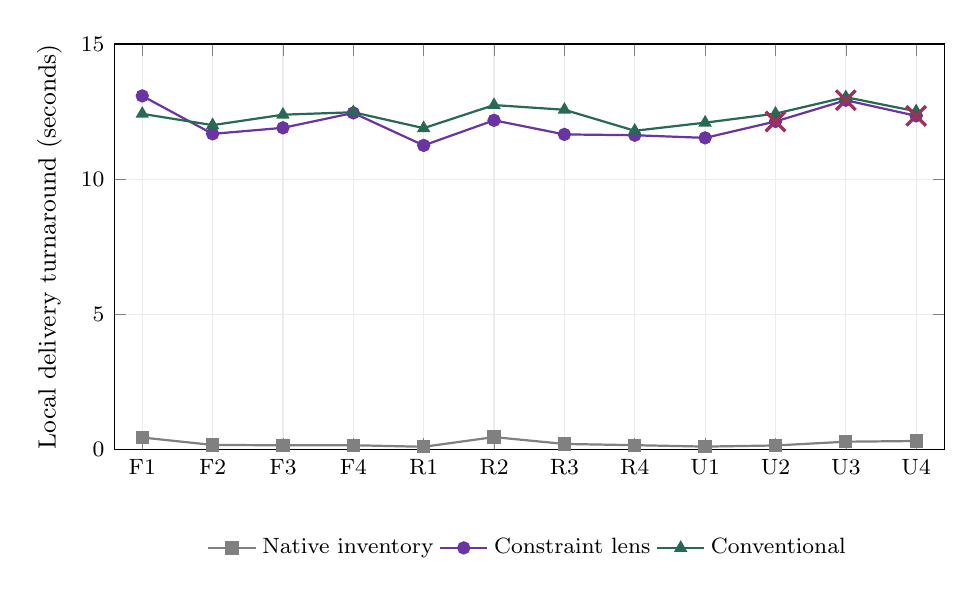
\begin{tikzpicture}
\begin{axis}[width=\textwidth,height=2.65in,ymin=0,ymax=15,xmin=.6,xmax=12.4,
ylabel={Local delivery turnaround (seconds)},xtick={1,...,12},xticklabels={F1,F2,F3,F4,R1,R2,R3,R4,U1,U2,U3,U4},tick label style={font=\footnotesize},label style={font=\small},
legend style={at={(.5,-.19)},anchor=north,legend columns=3,font=\footnotesize,draw=none},grid=major,grid style={gray!15}]
\addplot[color=gray,mark=square*,line width=.8pt] coordinates {(1,0.4430) (2,0.1680) (3,0.1560) (4,0.1580) (5,0.1000) (6,0.4590) (7,0.2050) (8,0.1600) (9,0.1070) (10,0.1490) (11,0.2880) (12,0.3140)};
\addlegendentry{Native inventory}
\addplot[color=violet,mark=*,line width=.8pt] coordinates {(1,13.0810) (2,11.6760) (3,11.9000) (4,12.4500) (5,11.2490) (6,12.1780) (7,11.6560) (8,11.6260) (9,11.5280) (10,12.1350) (11,12.9210) (12,12.3430)};
\addlegendentry{Constraint lens}
\addplot[color=good,mark=triangle*,line width=.8pt] coordinates {(1,12.4170) (2,11.9990) (3,12.3860) (4,12.4760) (5,11.8870) (6,12.7420) (7,12.5680) (8,11.7910) (9,12.0910) (10,12.4240) (11,13.0340) (12,12.5110)};
\addlegendentry{Conventional}
\addplot[only marks,mark=x,mark size=5pt,color=rose,line width=1.2pt,forget plot] coordinates {(10,12.1350) (11,12.9210) (12,12.3430)};
\end{axis}\end{tikzpicture}
\caption{Median native Workbench delivery time across three order-rotated trajectories. F, R and U identify FastAPI, Requests and urllib3 transitions. Crosses mark custom-method admission failures. The native inventory is a less complete output; it does not include the unmeasured human work needed to finish the packet. These shared-host timings are descriptive, not a human savings ratio or a capacity guarantee.}
\end{figure}

\subsection{Ablation and negative controls}
The original native inventory/diff arm is an executed capability ablation: it preserves its existing tools but does not supply a binding decision. A separate, disclosed development ablation removes the captured consumer code while retaining source comparison and independent verification. The upstream losses remain, but the historical exact forwarding call cannot be identified. The cheaper reduced-scope result therefore does not satisfy the same customer outcome. Its measured resources and original output are preserved separately; it is not relabelled held-out confirmation.

Development checks cover changed-source and stale-asset identity, cache tampering, malformed reports, false witnesses, constructors, positional-only arguments with variadic keywords, conditional/rebound definitions, source bounds, unchanged-source no-ops and native artifact integrity. Seventy-five shared tests and 47 candidate cross-checks passed before acquisition, including 150 seeded synthetic signature pairs inside a test. They are controls, not customer workloads. Original failed development attempts, the metadata-only fairness correction and the later primary rejection remain in the package.

\section{Complete cost, human work and a credible price}
\subsection{What has actually been measured}
Execution uses no runtime model or network call in the registered assessment worker. This does not make construction, hosting or the full service free. The complete confirmation campaign used \CampaignWall\ seconds elapsed and \CampaignCPU\ observed child-process CPU seconds, including the workers, independent verification, serialization and native pack construction. It includes 108 experimental evaluations, which must not be used as paid utilization. The complete successful offline support replay separately took 18.634 seconds and 18.590 child-process CPU seconds. Source acquisition, earlier failures, experimental comparisons, documentation and publication are additional recorded work.

Per-mission reporting distinguishes measured CPU/elapsed time, source and consumer bytes, requests, cache activity and validation from unknown money charges. Worker analysis time is not the same as total native delivery turnaround. The native \pathcode{reviewMinutes: 1} field declares template review capacity; it is not measured human attention. The study does not multiply elapsed assistant time by a wage or infer an inference bill from wall time. Model construction, tool overhead and future maintenance remain unpriced; a finite defensible upper bound was not available.

\begin{table}[H]\small
\begin{tabularx}{\textwidth}{@{}p{1.28in}Yp{1.1in}@{}}\toprule
Cost view & Included obligations & Monetary result\\\midrule
Marginal execution & Intake, source processing, caller mapping, verification, retries, packaging and residual exceptions for one accepted scope & \unknown\\
Recurring delivery & Marginal execution plus attributable hosting, retained storage, idle capacity, shared maintenance and business costs at declared utilization & \unknown\\
Fully loaded & Recurring delivery plus attributable discovery, unsuccessful candidates, construction, integration and maintenance investment over a justified horizon & \unknown\\\bottomrule
\end{tabularx}
\caption{Unknowns are retained in the canonical ledger. CPU time, a no-fee software license or zero runtime model calls cannot supply the missing complete monetary totals.}
\end{table}

Input registration and pipeline execution are automated. Supplying the correct public consumer scope and proposed revisions is customer setup; confirming application behavior and interpreting unresolved evidence remain genuine customer/reviewer work. The historical minimal probe, known-remedy integration and final presentation were supplied during this research session. Shared maintenance includes changed language/library semantics, export-resolution rules, source supply and tool versions. These activities cannot be assumed to vanish at scale.

\subsection{Comparison with competent work without AI}
The U.S. Bureau of Labor Statistics reports a May 2025 median hourly wage of USD 50.14 for software quality assurance analysts and testers \cite{bls-wage}. The Government of Canada Job Bank reports a Montréal median of CAD 46.26 per hour for the relevant broader information-systems occupation, based on 2024 data and updated 19 November 2025 \cite{jobbank}. These are wage benchmarks, not invoices or measured task durations. A broad professional-occupation benefits ratio from June 2026 BLS compensation data would yield an explicitly modelled USD 72.48/hour QA figure; it is not observed occupation-matched compensation \cite{bls-ecec}. The primary comparison uses the wage-only rate and keeps currencies separate.

For an equal accepted scope, let $h$ be the competent human's minutes, $w$ the appropriate hourly cost, $P$ the proposed customer price and $E$ the value of additional customer effort relative to the alternative. Customer advantage requires
\[
             P + E < \frac{wh}{60},
\qquad h > \frac{60(P+E)}{w}.
\]
At the sourced U.S. wage benchmark, each USD 1 of price plus additional effort requires more than 1.19665 minutes of equivalent human work to cross this wage-only threshold. At the Montréal benchmark, the separate CAD threshold is 1.29702 minutes per CAD 1. This is algebra, not an observed saving. Task duration, remaining effort, quality and responsibility must match before a savings ratio is reported.

No same-scope customer price is established. The broader advertised assessment and free tools show why upgrade work can matter commercially, but neither supplies our willingness-to-pay distribution. Consequently there is no supported numerical customer saving or margin to report. The bilingual demonstration offers a calculator with blank price, effort and cost inputs; any user-entered result remains a labelled scenario and never changes the actual ledger.

\section{Does the tested investment pay back?}
The cost and financing adapters use byte-identical canonical Alpha accounting modules from the existing integration source candidate. They preserve starting capital, actual collections, delivery costs, unpaid obligations, reserves and available surplus as distinct quantities. This study observes zero customer collections and executes no financial transaction or new paid commitment. Construction resources exist; their outlay is unknown, not zero. Unknown capital and obligations cannot authorize a commitment.

For the same tested capability, let $I$ include discovery, failed construction, successful construction, validation and integration. Let $d_i$ be supported incremental delivery savings for the same accepted outcome, and $M(N)$ the incremental maintenance through $N$ genuine subsequent missions. Repayment requires
\[
       G(N)=\sum_{i=1}^{N}d_i-I-M(N)\geq 0.
\]
The custom method's three failed scope admissions and all comparator construction belong in this finite accounting. No unrelated hypothetical capability is financed. If a constant net saving $d-m$ were supported, the arithmetic crossing would be $\lceil I/(d-m)\rceil$ for $d>m$; otherwise savings do not supply finite repayment. Here the complete $I,d,m$ and justified paid volume are unidentified. The canonical horizons of 1, 4, 12, 52 and 250 reuses are explicitly assumed sensitivity axes, not observed demand. Low utilization, higher maintenance, failures and absent demand cannot rescue that missing evidence.

The correct economic decision is \textbf{HOLD: repayment not established}. This is not proof of negative net present value; it is refusal to manufacture a positive value from unmeasured attention, arbitrary pricing or accounting allocations. Internal customer savings are not enterprise receipts, and earlier completion is not additional eventual output. No second capability was financed from an alleged surplus. Better task support and reuse are observed locally; cheaper capability construction and sustained acceleration are not demonstrated.

\section{The smallest practical commercial test}
A further tiny parser optimization would not resolve the commercial question. The next test should use one real, currently pending dependency decision from an authorized maintainer and the exact free-tool alternative the maintainer already uses. Freeze the code scope, acceptance and review question before examining the output. Deliver both packets, record whether the maintainer can identify a relevant code/test action, and measure the complete preparation, correction and customer-review effort. Preserve cases where both outputs are equally useful or the caller mapping cannot establish impact.

Collect actual metered infrastructure/model invoices for the offering boundary and attribute shared setup and maintenance at the observed utilization. With the same accepted responsibility, obtain a concrete buyer choice for a scoped paid pilot against the free alternative; that requires separate outreach or purchase authorization. No outreach, recruited panel, price offer or transaction was performed here. A single acceptance/usefulness test and a genuine purchasing choice are more decisive than a market-size multiplier. Total market size is therefore omitted: no serviceable or obtainable demand estimate is supported by this experiment.

\section{Integration, ecosystem and limits}
The new implementation is additive and local. It executes the unchanged native TI inventory and Workbench extension, keeps the native 200,000-code-unit artifact limit, and retains every source-admission refusal. Across the 138 before/after module slots, native inventory admits 35, refuses 102 and records one absent source. Refusals include narrow literal-source rules, credential-shaped-text screening and size limits. The separately labelled local research parser processes the permitted public snapshots without turning those refusals into native source-audit admission; this is a material integration limitation, not a production-qualified source service. Full evidence remains an external hash-bound companion artifact rather than being concealed behind an oversized native field. Packs have an unauthenticated historical status, explicitly labelled\\\pathcode{UNAUTHENTICATED_HISTORICAL_IMPORT}, with empty active authority, economic admission HOLD and settlement disconnected. An inert job-plan compilation is not an approved operator execution.

All four requested repositories were inspected. Alpha provides the executed local substrate; its embedded AGI Jobs compiler supplies the local plan path. Fleet and Manager supply relevant source/release and optional execution/settlement context, but neither a physical Fleet action nor a Manager settlement was needed. Source-level \$AGIALPHA utility includes route-specific escrow, staking, validation and reward machinery in Alpha/Jobs. The Manager route uses six-decimal USDC and its own escrow/bond/claim rules. No RPC or deployed-contract qualification was performed. These routes, token units and obligations are not interchangeable, and token holdings, issuance or appreciation are not operating profit or invented holder rights.

At the final read-only status check (14:02:37 UTC), Alpha main was at \pathcode{804e1afe} (full identity in the final status record); the public v1.43.0 tag still identified an earlier source revision. The exact experimental-source release-acceptance run 40323676127 remained in progress, with no conclusion. Fleet and Jobs were public prereleases; Manager v1.20.2 remained a separate release. The timestamped final status record is included.

The four earlier economic studies, their source editions, negative findings and original URLs are preserved \cite{awe,next-advantage,funded-advantage,investment-gate}. Overnight checksum and bounded-retry work is audited as merged source with limited prior evidence, not automatically a released or production-qualified service. The other writer's recurring repair-admission and validation-cost lane is not duplicated. Security, binary-admission, exact-source, owner-review, operator and publication gates remain independent of this study's local checks.

The main limitations are narrow static semantics, incomplete caller resolution, three historical package clusters, possible training exposure, one exposed runtime incident, same-session review, unknown human/monetary inputs and no paid demand. The strong comparator's conservative scope agreement is not proof of semantic superiority. The publication overlay is additional work beyond generic automatic output. These limitations delimit the offering and its price test; they do not erase the useful historical result or excuse inflation into a self-financing enterprise.

\appendix
% Technical appendix fragment; no document preamble and no outcome/price claims.
% Uses ordinary LaTeX plus amsmath. Integrate before the bibliography.
% Source: frozen implementation and development records only.
\section{Source-bound dependency decisions: technical methods}
\label{app:binding-methods}

This contribution adds argument-binding evidence and consumer-call triage to
source-pinned dependency assessment. It is separate from recurring repair
admission or validation-cost optimization. Its endpoint is a bounded decision
artifact: identify the declarations and captured calls requiring review,
provide replayable binding counterexamples, and retain explicit uncertainty.
A binding result is neither application compatibility nor upgrade approval.

\subsection{Declared object and execution boundary}

The declaration model includes direct, undecorated, top-level functions with
non-underscore names, including asynchronous functions, and qualified direct
\texttt{PublicClass.\_\_init\_\_} declarations. Constructors must be synchronous
and undecorated; their classes must be undecorated, have at most one explicit
base, and have no class keywords or metaclass declaration. Duplicate,
conditional, rebound or imported replacement bindings remain unresolved.
Dynamic module constructs, including star imports, module
\texttt{\_\_getattr\_\_}, and recognized active
\texttt{exec/eval/globals/locals} calls, also prevent a resolved declaration
claim. These syntactic checks do not establish general runtime namespace
stability or that a declaration in an internal module is a supported public
API.

The declared per-source limits are 1,000,000 UTF-8 bytes, 100,000 AST nodes,
and 64 parameters per callable. Parsing, scope or resource refusal is recorded
as unresolved. The existing native source-inventory path retains its own
tighter admission limits; a successful local analysis does not override a
native refusal. Unchanged source identities are no-ops rather than new
missions. Source identities, changed/unchanged inventories, omissions and
refusals remain in the dossier.

Inspected source is parsed, never imported or executed by the binding tools.
Original bodies, decorators, annotations, type parameters and default
expressions are excluded from executable stubs. Optional defaults become
constant \texttt{None}, and a generated body only returns \texttt{None}.
Default-expression text may be retained as inert metadata. Separately
authorized integration experiments on pinned published packages execute
those packages under their declared isolation controls; that is a different
evidence layer and is not silently implied by a static report.

\subsection{Finite binding domain and containment theorem}

Represent a call shape as $(n,K)$: $n$ positional arguments and a finite set
$K$ of distinct keyword names. Values are immaterial to Python argument
binding once argument evaluation succeeds. Duplicate keyword production or
failed argument evaluation occurs outside this model.
Let $s_0$ and $s_1$ be the before and after signatures. Let $P$ be their maximum
number of fixed positional parameters, and let $U$ contain all parameter
names in either signature plus one fresh name occurring in neither.
The finite domain is
\[
  D = \{0,\ldots,P+1\}\times\mathcal{P}(U),
  \qquad |D|=(P+2)2^{|U|}.
\]
The endpoint asks whether every before-accepted shape is also accepted after.
The absence of a supported local declaration is treated as an empty local
binding language only when the scope checks exclude an unresolved
replacement; it is not proof about package exports.

For signature $s$ at fixed $n$, first reject positional infeasibility: too
many positional arguments without \texttt{*args}, or an unfilled required
positional-only parameter. Otherwise define $R_s(n)$ as the unfilled required
positional-or-keyword names together with required keyword-only names.
Define $A_s(n)$ as all keyword-eligible names, excluding
positional-or-keyword names already filled positionally. With
\texttt{**kwargs}, every name in $U$ is eligible before that exclusion.
Without it, only unfilled positional-or-keyword and keyword-only names are
eligible. Thus
\[
 (n,K)\text{ binds to }s
 \quad\Longleftrightarrow\quad
 n\text{ is feasible and }R_s(n)\subseteq K\subseteq A_s(n).
\]

\paragraph{Containment proposition.}
For each $n$ admitting a before call, containment holds exactly when the
after signature is feasible and
\[
 R_{s_1}(n)\subseteq R_{s_0}(n),
 \qquad A_{s_0}(n)\subseteq A_{s_1}(n).
\]
If the after signature is infeasible, requires a keyword absent from the
before minimum, or rejects a keyword in that minimum, then
$K=R_{s_0}(n)$ is a counterexample. Otherwise any
$x\in A_{s_0}(n)\setminus A_{s_1}(n)$ yields the counterexample
$K=R_{s_0}(n)\cup\{x\}$.

\paragraph{Proof and finite reduction.}
The accepted keyword sets at fixed $n$ form the interval
$[R_s(n),A_s(n)]$ under set inclusion. The minimum before set tests every
after requirement; one-key extensions test every possible after prohibition.
There are no additional cross-key constraints for distinct keyword names.
For $n>P$, both signatures have exhausted their fixed positional slots, so
every greater count has the same accept/reject behavior determined by
\texttt{*args}; $P+1$ therefore represents that entire tail. Names outside
the union of parameter names have identical binding behavior, determined
only by \texttt{**kwargs}. Any separating set containing such names can
replace them by the one fresh representative. Consequently a loss anywhere
in the ordinary binding-shape language has a witness in $D$, and the stated
minimum-plus-singleton frontier suffices. This establishes a property of the
declared signature model, not behavior, type compatibility or business value.

The retained implementation, \texttt{src/dossier.py}, computes these
constraints directly. Witnesses contain only a positional count and sorted
keyword names, so they can be replayed against inert stubs with constant
argument values. An unchanged binding language may still hide changed
defaults, positional meaning, return values, side effects or an asynchronous
contract; warnings do not turn those untested properties into guarantees.

\subsection{Independent evaluation and strong conventional comparison}

\texttt{src/validate\_dossier.py} independently inventories declarations with
an AST visitor and independently renders safe stub source. It checks module
and source identities, exact declaration inventory, signature metadata,
reported states, coverage reconciliation, findings and every supplied
counterexample. Stub calls exercise CPython's actual binder.
\texttt{inspect.signature} is used on generated stubs for metadata;
\texttt{Signature.bind} is not the binding oracle.

For small domains the evaluator enumerates all positional counts and
keyword subsets. Identical generated binding signatures permit an exact
equivalence shortcut. In default automatic mode, a domain exceeding the
remaining one-million-shape budget uses a separately implemented complete
minimum-plus-singleton frontier. Each check records its method. Explicit
exhaustive mode does not use this fallback; exhausted budgets remain unknown.
A verified concrete counterexample can prove a loss even when full
enumeration is unaffordable. Report correctness and complete supported-scope
coverage are separate fields: an honest unresolved report is not a complete
compatibility finding. Independent code and extraction reduce common
implementation failure, but the same Python runtime and the frontier
theorem remain shared assumptions; this is not an external blinded audit.

The strong conventional arm, \texttt{src/conventional.py}, uses the pinned
Griffe/griffelib 2.4.1 static visitor. It retains before/after snapshots and
all broader breaking-change alerts, then adds independently authored
safe-stub witness enrichment using the complete frontier. Griffe's metadata
label \texttt{runtime} is not evidence that inspected source executed.
Its broader alerts, including default and other API changes, remain available
for review and are not scored as false positives merely for falling outside
the narrow binding endpoint.

Both builders may retain reusable assets and legitimate caches. The
conventional cache includes source, module, implementation, runtime and
Griffe identities, with 64 entries and 16,000,000 captured source bytes;
that byte bound is not a process-memory limit. Returned objects are copied
to prevent consumer mutation of retained entries. The retained arm's disk
snapshots check source, implementation and serialized-fact identities.
Construction, failed attempts, cache operations and verification belong to
the resource record for the arm that incurred them. A free upstream tool is
not an assumption of free integration work. Declared cold/warm ablations
must not remove legitimate reusable assets only from the comparator.

\subsection{Constructor, keyword and consumer subtleties}

Positional-only names require particular care. For
\texttt{def f(x, /, **kw)}, the shape with one positional argument and keyword
\texttt{x} is valid: the positional argument fills the parameter and the
keyword enters \texttt{kw}. For
\texttt{def f(x, **kw)}, the same shape duplicates a binding and fails.
For \texttt{def f(x=0, /, **kw)}, a keyword \texttt{x} alone is also accepted
but does not fill the positional-only parameter. If that parameter becomes
required, the same keyword cannot satisfy it. Accordingly, only assigned
positional-or-keyword names are removed from $A_s(n)$; positional-only names
must not be removed when \texttt{**kwargs} can receive them.

Constructor comparison is of an unbound direct declaration, including its
receiver parameter. A consumer class call can add one implicit positional
receiver only under the declared direct-constructor assumptions.
\texttt{\_\_new\_\_}, metaclasses, runtime method resolution and constructor
behavior remain outside the claim. If a class remains but loses its direct
\texttt{\_\_init\_\_}, the result is unresolved because inheritance may
supply a constructor. It is not automatically a removed callable.

The shared \texttt{src/consumer.py} maps captured lexical imports and source
call sites. Literal tuple/list positional expansion and literal string-key
dictionary expansion can yield a shape; dynamic expansions, ambiguous
bindings, instance methods and unsupported dispatch remain unresolved.
The mapper handles qualifying single-base \texttt{super().\_\_init\_\_}
calls only conditionally. A separate candidate channel can follow captured
closed literal \texttt{\_\_all\_\_} exports, a recognized module-metadata
write pattern and narrowly screened import guards. These candidates do not
erase strict unresolved counts or establish runtime export identity.
Every mapped call assumes its imports and argument expressions succeed.

Both arms use this same consumer mapper and metadata contract. Its use of
the shared constraint helper makes this layer a common integration
component, not an independent validation of consumer runtime behavior.
Separate integration evidence is needed for that stronger conclusion.
Call-site counts, declaration counts and syntactic candidates are never
customer-job counts or measurements of independent defect recurrence.

\subsection{Development controls, freeze and preserved failures}

The frozen shared development suite contains 75 tests: 50 conventional and
evaluator tests, 20 consumer tests, and five pipeline tests. A further
crosscheck applies 47 of the shared conventional cases to the retained
implementation; these are reused controls, not 47 new observations from the
target workload. The three comparator-specific cases concern changed-source
cache invalidation, returned-object mutation isolation, and preservation of
broader Griffe alerts.

One shared test constructs 80 synthetic signatures using seed 2645 and
performs 150 sampled before/after pair evaluations. Those pair evaluations
are internal assertions within the development test and may reuse generated
signatures; they are not 150 independent missions. The suite also exercises
positional-only/variadic edge cases, inert defaults and bodies, constructor
exclusions, forged identities and metadata, malformed or omitted findings,
budget abstention, source-byte preservation, symlink refusal, native limits
and unchanged-source no-ops. Counts document controls rather than customer
acceptance or experimental sample size.

Original failures, development logs and superseded editions are retained.
Before confirmation exposure, a comparator metadata interoperability defect
was corrected: independently parsed signatures and ordered source identities
were added so the common consumer mapper could assess both arms. No candidate
comparison algorithm was imported. The original comparator freeze is
preserved under \pathcode{discovery/frozen-conventional-v1/}; the amendment is
recorded in \pathcode{discovery/conventional-freeze-v2.json}. Source identities
and the final protocol are fixed by
\texttt{discovery/final-freeze.json}. Subsequent confirmation failures must be
reported against that freeze, not repaired silently and relabeled untouched
confirmation.

The reproducible development entry point is:
\begin{verbatim}
PYTHONPATH=src:deps/site python3 -m unittest discover \
  -s tests -p 'test_*.py' -v
\end{verbatim}
Run it from the companion root with the retained pinned dependencies.
The historical integration runner and its original bounded failures are a
separate development artifact; they do not increase the confirmation sample
or establish deployment qualification.


\section{Reproduction and exact-source record}
The complete companion includes original sources and licenses, frozen protocol/implementations, all outcomes and failures, machine-readable resources and financing records, dependency wheels, the bilingual demonstration and verification support. A clean offline replay installed twelve hash-pinned runtime distributions, confirmed zero missing dependencies and imports from the new environment, ran the 75 shared and 47 candidate controls, executed the canonical economics tests and reproduced the native historical packet. Its result and the earlier staging failure are preserved.

\begin{verbatim}
python3.12 support/replay_offline.py \
  --out /tmp/agi-alpha-replay-001 \
  --mission httpx-development --arm conventional

# From the companion root, after setting up the verified environment:
node src/workbench.mjs httpx-development conventional results/new-run
node src/campaign.mjs results/new-confirmation
\end{verbatim}

The new-run commands write separate raw execution records. The study summarizer reads the preserved primary campaign at its fixed path; it does not analyze a new campaign directory. See the reproduction guide before regenerating derived records, and retain the sealed original archive.

The supplied wheel boundary is CPython 3.12, Linux x86-64, glibc at least 2.34. The observed environment used Python 3.12.14, glibc 2.39 and Node 24.22.1; the repository's separate Node 22.17.1 qualification requirement is not claimed satisfied. The operating system, Python/venv/ensurepip and Node remain prerequisites. The full platform/release campaign was not run. The new local-source registration utility accepts explicit snapshots and commits; supplied commit labels alone do not prove remote Git custody, so independently verified source provenance remains part of acceptance.

\begin{table}[H]\footnotesize
\begin{tabularx}{\textwidth}{@{}p{1.45in}Y@{}}\toprule
Identity & Frozen value / role\\\midrule
Alpha experimental source & \pathcode{eb07086ac42799ff45f7b1c946a2f7c514bd3bbc}\\
Canonical accounting source & \pathcode{496fa3c00dc7498173a896404ec756dfdeb94033}; existing open integration candidate, not released adoption\\
Protocol SHA-256 & \pathcode{6f0d07a2d310cf6a1cf92b3c8b6033fd3366295872ca2bce9ac2888342661689}\\
Exact freeze SHA-256 & \pathcode{25ee20b1cd68710a5eea65fc08e2eba2f47a521bfde2d9ebbf37731280bc6d64}\\
Held-out metadata SHA-256 & \pathcode{eeddceae75c6b10c97369da9baff2fc69928e9e9fe3c0025499c2529e846160e}\\
Source custody SHA-256 & \pathcode{73adee1cd52ec8477a240b4e7b855038d925d0bdee8ad9c6b403596a6c6f0ee2}\\\bottomrule
\end{tabularx}
\caption{Exact hashes are machine-checked in the companion; the public freeze comment supplies a coordination timestamp, not an independently audited proof of absence of training exposure.}
\end{table}

\section{Accounting and intervention register}
All research was performed by AI-assisted authors under user direction, with separate agents constructing the comparator, reviewing sources and economics, and auditing outcomes. The constructor was not an autonomously deployed enterprise. Human contributions include the user's objectives/steering and the pre-existing upstream repair; actual research-model billing and the user's attention are not measured. The complete research cost includes rejected opportunity screening, failed development controls, the custom candidate, comparator construction, metadata/schema integration, source acquisition, verification, recovery, publication and packaging. Timestamps and observed compute are retained without converting them into a bill.

The canonical ledger charges capability construction once to a named investment account, not once per mission. Its accepted mission entries mean internally validated scoped research packets, not paid customer acceptance. The cost model's required base/conservative/stress names all retain unknown inputs; they are not invented favorable forecasts. No simulated receipts are substituted for actual zero collections. No funding, reinvestment transaction, token purchase, distribution, buyback, credential, persistent access expansion or security-setting change was performed.

\begin{thebibliography}{99}\small\raggedright
\bibitem{starlette-discussion} Starlette maintainers and community. \emph{HTTPX 0.28 incompatibility with Starlette TestClient}, discussion 2770 (historical). \url{https://github.com/Kludex/starlette/discussions/2770}.
\bibitem{httpx-release} HTTPX maintainers. \emph{HTTPX 0.28.0 release}. \url{https://github.com/encode/httpx/releases/tag/0.28.0}.
\bibitem{starlette-release} Starlette maintainers. \emph{Release notes, 0.37.2}. \url{https://www.starlette.io/release-notes/#0372-march-5-2024}.
\bibitem{netlandish} Netlandish. \emph{Django upgrades: assessment and implementation service}. Retrieved 26 October 2026. \url{https://www.netlandish.com/services/django-upgrades/}.
\bibitem{griffe} Griffe maintainers. \emph{Checking for breaking changes}; implementation pinned to 2.4.1. \url{https://mkdocstrings.github.io/griffe/guide/users/checking/}.
\bibitem{github-pricing} GitHub. \emph{Plans and pricing}. Retrieved 26 October 2026. \url{https://github.com/pricing}.
\bibitem{renovate} Mend. \emph{Renovate Community Cloud and resource tiers}. Retrieved 26 October 2026. \url{https://docs.mend.io/renovate/latest/mend-renovate-cloud-resource-tiers}.
\bibitem{bls-wage} U.S. Bureau of Labor Statistics. \emph{May 2025 occupational wage estimates, national table}, software quality assurance analysts and testers (15-1253). \url{https://www.bls.gov/news.release/ocwage.t01.htm}.
\bibitem{bls-ecec} U.S. Bureau of Labor Statistics. \emph{Employer Costs for Employee Compensation, June 2026, Table 4}, professional and related occupations. \url{https://www.bls.gov/news.release/ecec.t04.htm}.
\bibitem{jobbank} Government of Canada, Job Bank. \emph{Information systems specialist wages, Montréal}, NOC 21222; 2024 reference, update 19 November 2025. \url{https://on.jobbank.gc.ca/marketreport/wages-occupation/22511/geo25154}.
\bibitem{freeze} AGI ALPHA research coordination. \emph{Issue 4850: exact pre-confirmation freeze}, comment 6417289596, 26 October 2026. \url{https://github.com/MontrealAI/AGI-Alpha-Agent-v0/issues/4850#issuecomment-6417289596}.
\bibitem{awe} AGI ALPHA. \emph{The Autonomous Work Economy}, preserved edition. \url{https://github.com/MontrealAI/AGI-Alpha-Agent-v0/blob/main/docs/papers/agi-alpha-autonomous-work-economy-v1.pdf}.
\bibitem{next-advantage} AGI ALPHA. \emph{Build the Next Advantage}, preserved edition. \url{https://github.com/MontrealAI/AGI-Alpha-Agent-v0/blob/main/docs/papers/agi-alpha-next-advantage-v1.pdf}.
\bibitem{funded-advantage} AGI ALPHA. \emph{The Advantage That Funds the Next}, preserved edition. \url{https://github.com/MontrealAI/AGI-Alpha-Agent-v0/blob/main/docs/papers/agi-alpha-funded-advantage-v1.pdf}.
\bibitem{investment-gate} AGI ALPHA. \emph{The Investment Gate}, preserved edition. \url{https://github.com/MontrealAI/AGI-Alpha-Agent-v0/blob/main/docs/papers/investment-gate.pdf}.
\bibitem{alpha-source} MontrealAI. \emph{AGI-Alpha-Agent-v0}, exact experimental source. \url{https://github.com/MontrealAI/AGI-Alpha-Agent-v0/tree/eb07086ac42799ff45f7b1c946a2f7c514bd3bbc}.
\bibitem{fleet} MontrealAI. \emph{AGI-Fleet-Linux}, inspected source 45759fb096faf8988f58ae5ea71248d0f35a97c7. \url{https://github.com/MontrealAI/AGI-Fleet-Linux}.
\bibitem{jobs} MontrealAI. \emph{AGIJobsv0}, inspected source bc4abbd5c28f3672275b13300e40ea26c820b8ee. \url{https://github.com/MontrealAI/AGIJobsv0}.
\bibitem{manager} MontrealAI. \emph{AGIJobManager}, inspected source 5d5670df9dbbc79da115e0a44b71989f34df58c1. \url{https://github.com/MontrealAI/AGIJobManager}.
\end{thebibliography}
\end{document}
